\chapter{Introduction}
\label{chapter:body}
\thispagestyle{myheadings}
\setcounter{tocdepth}{1}
% set this to the location of the figures for this chapter. it may
% also want to be ../Figures/2_Body/ or something. make sure that
% it has a trailing directory separator (i.e., '/')!
\graphicspath{{1_Intro/Figures/}}

Incoherent scatter radar (ISR), like all scientific instruments, is a testament to humankind's desire to understand the world around it. This is especially true for ISR because these systems are generally very large, complicated and use substantial amounts of power, in the range of megawatts at peak levels. These systems are able to probe Earth's ionosphere and, unlike other ground-based measures, this modality can give direct measurements of various ionospheric plasma parameters including electron density ($N_e$), electron temperature ($T_e$), ion temperature ($T_i$) and ion velocity ($V_i$). ISRs have been in use since the 1950's \citep{gordon58} and these systems have evolved over time from only being able to measure parameters along a single line of sight to recently having the ability to be used as full 3-D sensors \citep{Semeter2009738,Nicolls:2007ie}. The goal of this dissertation is to present a framework to analyze and improve the quality of the data that comes from modern ISR systems. This framework can  improve the spatial and time sampling of the ISR systems and help researchers improve their experiments and better understand the data products from ISR.

Until recently, ISR systems were constructed using single, mechanically steered antennas. With this approach, the rate that the look angle can change is limited by the mechanical speed of the antenna steering mechanism. The newest generation of ISR systems now take advantage of electronically steerable array (ESA) antennas, which allow for a near instantaneous change in the radar look direction. While this thesis mainly focuses on ESA ISR systems, many of the ideas contained within are also applicable to experiment design for ISR systems with single mechanically steered antenna.. 
 
\section{Purpose}
The basics of ISR will be introduced in the following section along with recent developments expanding ISR capabilities. The ionosphere and ISR observable characteristics will then be discussed. Finally the section will close with a short introduction to inverse theory and image reconstruction as used by engineers and scientists to analyze and improve the output of sensors.

\subsection{ISR as a 3-D Sensor}
Radar is a common remote sensing modality that has found diverse uses ranging from mundane supermarket door openers and traffic speed control~\citep{richards2010principles} to mapping the surfaces of planetary bodies~\citep{campbell2002radar}. ISR systems estimate plasma parameters via radiating electromagnetic energy and monitoring the reflected signal from large groups of free electrons in the ionosphere. The monitoring of radar returns may take place at the transmitter site (monostatic) or at one or more distinct receive locations in bistatic or multistatic systems~\citep{RDS:RDS2903}. The plasma-scattered radar energy has a specific spectral distribution statistics dictated by the ion and electron temperature, electron density and bulk flow of the plasma in the measured ionospheric volume~\citep{dougherty:farley1960,farleydougherty:ISR2,doughteryfarley:ISR3,hagfors1961}. Two important steps in ISR processing are:
\begin{enumerate}
\item estimation of a power spectrum or equivalently, an autocorrelation function (ACF)~\citep{farley1969}
\item fitting measured ACFs or spectra to a physics based model with plasma parameters as inputs~\citep{RDS:RDS1387}.
\end{enumerate}
This process is executed at each point in time and space where the radar can create an ACF estimate~\citep{nikoukar2008}. 

As stated previously, ESA antennas can create three dimensional reconstructions of plasma parameters. Examples of ESA ISRs include Advanced Modular Incoherent Scatter Radars (AMISR).
As the name implies, AMISRs can be built with varying numbers of panels and can be relocated. Each of these panels contain 32 antenna element units.
Full 128-panel AMISR sites are currently deployed to Poker Flat Research Range north of Fairbanks, Alaska and Resolute Bay, Nunavut, Canada~\citep{Semeter2009738,Valentic:2013jg,Nicolls2015a}. These systems are constructed into a roughly 30$\times$30 meter square face.
Smaller sixteen-panel AMISRs are deployed to Gakona, Alaska (HAARP site) and Arecibo, Puerto Rico.
The Poker Flat Incoherent Scatter Radar (PFISR) is depicted in Figure~\ref{fig:amisrpic}, with Resolute Bay Incoherent Scatter Radar (RISR) having similar construction. 
These systems have already yielded unprecedented views in the ionosphere and upper atmosphere and allowed for new types of measurements that were not possible before \citep{semeter2010CI,butler:imagingfregiondrifts,Nicolls:2007ie}. %Currently EISCAT-3D is being developed as well and is expected to give even greater views due to the multi-static set up \citep{eiscat3ddesign}.

%\begin{figure}[!t]
%\centering
%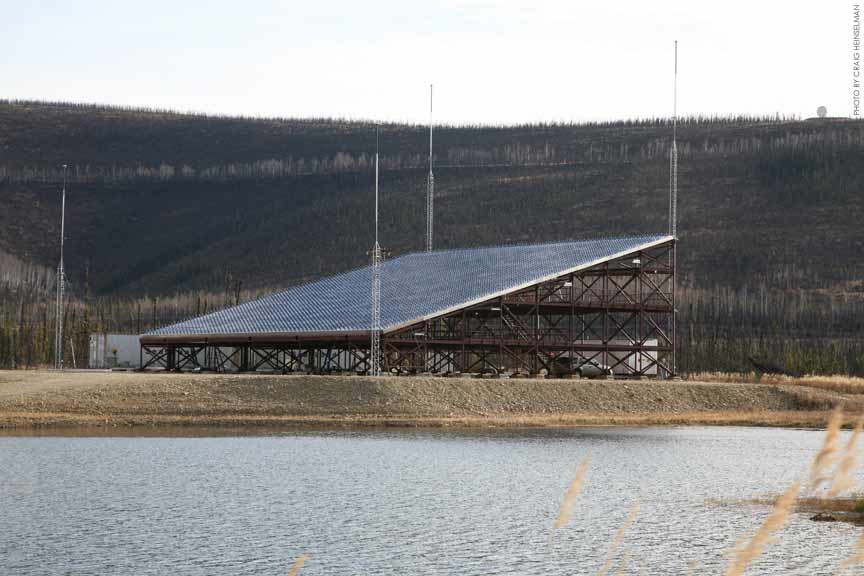
\includegraphics[width=3in]{amisrimage2}
%\caption{PFISR field deployment at Poker Flat Research Range~\citep{Valentic:2013jg}}
%% * <mhirsch@bu.edu> 2016-11-14T17:41:02.369Z:
%%
%% perhaps add a physical scale reference to give a sense of the size e.g. 30 meters or whatever
%%
%% ^.
%\label{fig:amisrpic}
%\end{figure}

\begin{figure}[htb]
  \begin{minipage}[t]{0.49\linewidth}\centering
    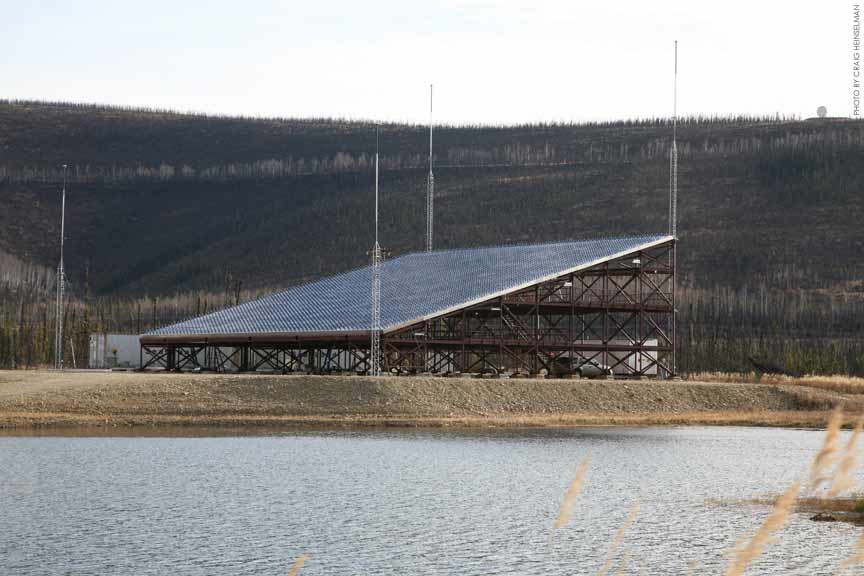
\includegraphics[width=7cm]{amisrimage2}
    \medskip
    \centerline{(a)}
  \end{minipage}\hfill
  \begin{minipage}[t]{0.49\linewidth}\centering
    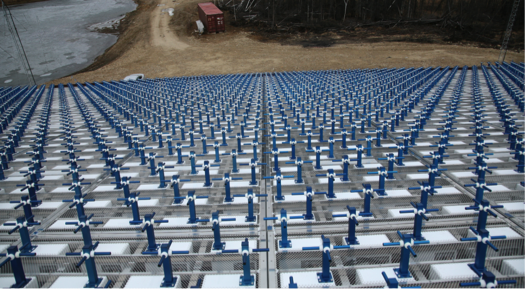
\includegraphics[width=7cm]{amisrface}
    \medskip
    \centerline{(b)}
  \end{minipage}
  \caption{PFISR field deployment at Poker Flat Research Range~\citep{Valentic:2013jg}: (a) View of full system, approximately 30$\times$30 meter; and (b) Close up view of the individual cross dipole antenna elements units. }
  \label{fig:amisrpic}
\end{figure}

\subsubsection{Objectives related to 3-D ISR}
A large and growing number of studies have used ISR to reconstruct two- and three-dimensional fields of plasma parameters. Some studies use various types of interpolation to stitch together a spatially-continuous parameter estimate from the sparse angularly-sampled one dimensional beams, which give a one dimensional view along range \citep{Semeter2009738,Butler:2013ul,Semeter:2005fo}. Others have taken an approach similar to inverse theory and image reconstruction to create estimations of velocity fields of bulk flows or electric fields \citep{butler:imagingfregiondrifts,RDS:RDS20195}. These publications, typically, do not describe the core details of reconstructing plasma parameters, such as the ion and electron temperatures. Interpolations can help visualize the data, the analysis used makes a large number of assumptions about the underlying imaging process. The goal of this thesis is to present a first-principles model of ISR as a three dimensional sensor and to use the model to create better reconstructions of the plasma parameters.
% * <mhirsch@bu.edu> 2016-11-14T17:46:58.012Z:
%
% consider rephrasing positivity, something like the prior work interpolates but here we use inverse theory instead of just smearing numbers together
%
% ^.

\subsection{Ionosphere and Phenomena}
The ionosphere is the area of partially ionized gas, or plasma, surrounding the earth, and presents a conductive lower boundary to ionized particles from the magnetosphere and solar wind~\citep{kellybook}. The dynamics of this system are governed by kinetic, fluid and Maxwell's equations coupled together \citep{schunk2004ionospheres}. This complicated menagerie of equations allows for the creation of a cornucopia of different phenomena at any number of spatio-temporal scales \citep{Semeter:2008hs,Semeter2009738}.

%In order to understand the behavior of the plasma in the ionosphere one needs to use electromagnetic theory governed by Maxwells Equations seen in Equations \ref{eqn:max1} and \ref{eqn:max2},

%\begin{eqnarray}
%\label{eqn:max1}
%\nabla \cdot \vec{E} = \frac{\rho}{\epsilon_0}\  &&\nabla  \cdot \vec{B} = 0 \nonumber \\
%\nabla  \times \vec{E} = - \frac{\partial B}{\partial t} && \nabla  \times \vec{B} = \mu_{0}\vec{J} +
%\mu_{0}\epsilon_{0}\frac{\partial E}{\partial t}
%\end{eqnarray}
%
%\begin{equation}
%\label{eqn:max2}
%\frac{\partial \rho}{\partial t}+\nabla \cdot \vec{J} = 0
%\end{equation}
% 
%\noindent where $\rho$ is the charge density, $\vec{E}$ is the electric field, $\vec{B}$ is the magnetic field, $\vec{J}$ is the current density, $\mu_0$ is the vacuum permeability and $\epsilon_0$ is the vacuum permittivity. 
%
%In order to close the system of equations often assumptions about the charge density and current density are needed \citep{varnytalk2016}. In the ionosphere though $\vec{J}$ is linked to the electric and magnetic fields, $\vec{E}$ and $\vec{B}$, which are dependent on the particle motion. In the ionosphere these particles move as gas, so to close these systems of equations require the use of fluid and/or kinetic theory depending on what sort of assumptions can be made for the problem.

The study of the Earth's ionosphere is typically broken up into several regions with distinct physical processes that dominate each region~\citep{kellybook}. Demarcations between the D, E and F Regions are based on altitude, over which various properties of the plasma, including parameters and chemical composition, can greatly vary as shown in Figure \ref{fig:singlefilt} \citep{kellybook}. The regions of the Earth are also parceled out based on the orientation of the magnetic field to the ground and include the polar caps, auroral oval, mid latitude, low latitude and magnetic equatorial regions~\citep{schunk2004ionospheres}.

For this thesis, most of the focus will be on phenomena from the auroral and polar cap F-region ionosphere. In this region, distinct phenomena arise related to the nearly-perpendicular angle of the Earth's magnetic field to the ground \citep{schunk2004ionospheres}. These phenomena include but are not limited to aurora borealis, polar cap plasma patches and particle precipitation events \citep{Perry:2015jf,Dahlgren:2013ip,dahlgren2012di,Dahlgren:2012dq,semeter:plasmatransport2012}. From a societal standpoint, this sort of activity can greatly impact radio propagation and can create interruptions in navigation and timing services such as the Global Navigation Satellite Systems (GNSS) including Navstar GPS, Galileo, GLONASS, Beidou \textit{et al}~\citep{Jiao:2013ei,hunsucker2007high}.


\begin{figure}[!t]
\centering
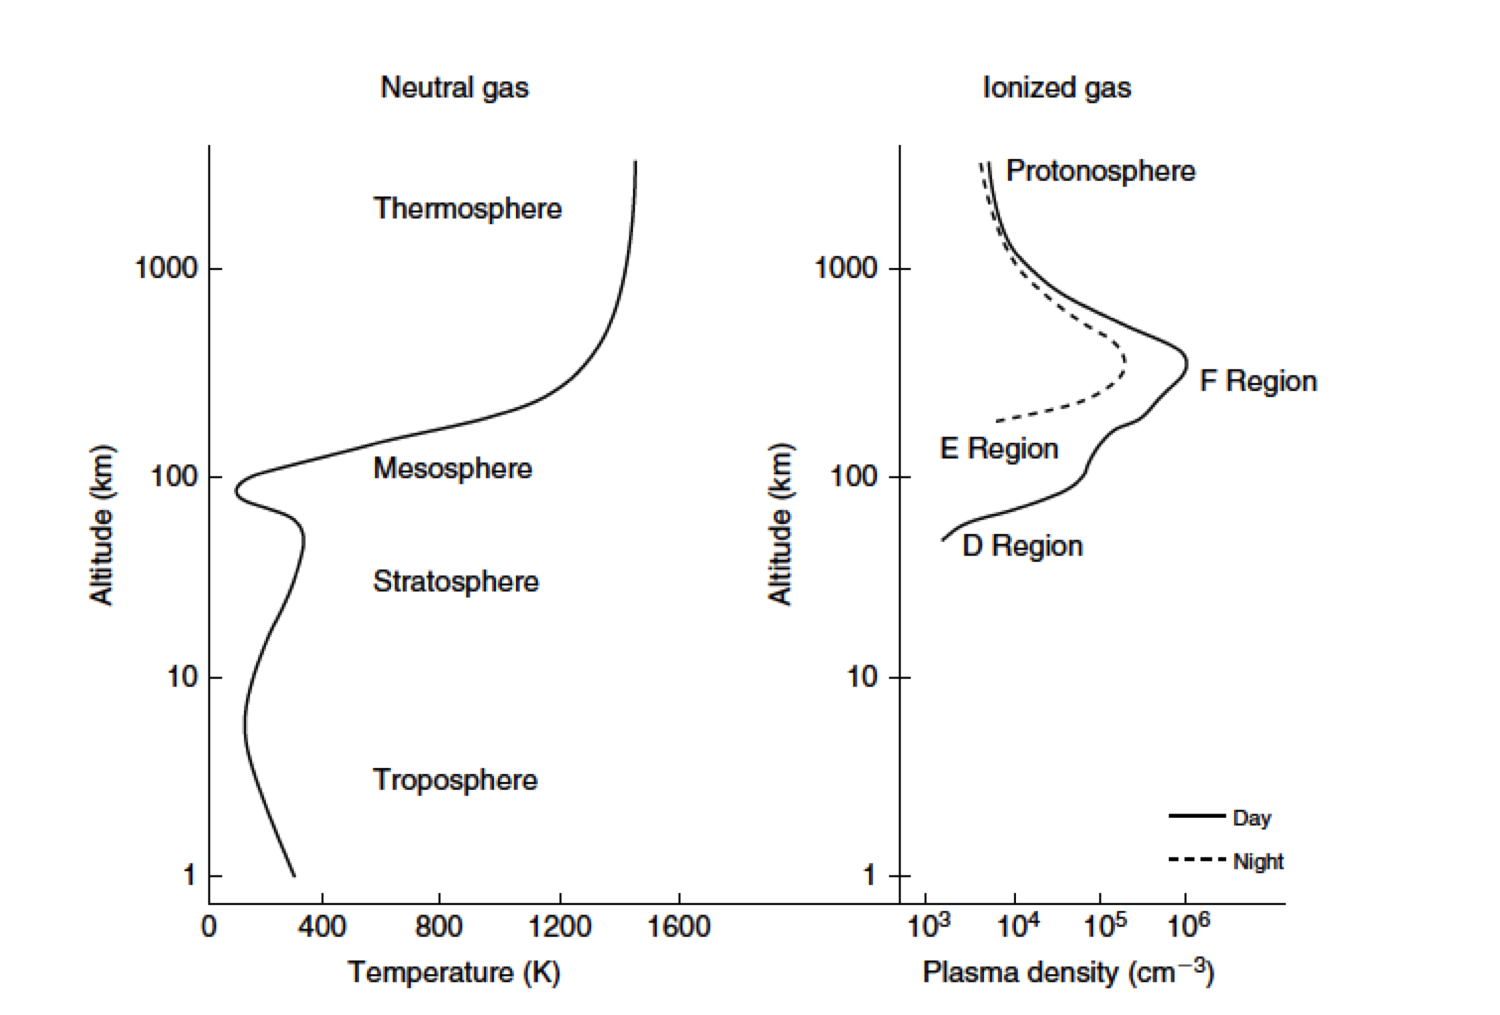
\includegraphics[width=5in]{altvsparams}
\caption{Example profiles of (left panel) neutral temperature and (right panel) plasma density from \citet{kellybook}}
\label{fig:singlefilt}
\end{figure}
%These systems right now are all located in what can be considered the high latitude ionosphere.  This is a highly dynamic environment in both time and space.  The plasma can change very quickly due to the physics of the environment.  These types of events can be classified into a number of types that will be of interest to this type of sampling problem.

%\subsubsection{High Spatial Gradient Events}
%Polar cap patches are examples where of high spatial gradients in various plasma parameters \citep{Dahlgren:2012dq,dahlgren2012di}.  In the polar cap large blobs of plasma with elevated electron density travel from the dayside to the night side ionosphere.  These patches can play a large role in plasma transport within the polar ionosphere and interfere with radio transmission as well.  Examples of sensor data that show these patches can be seen in Figure \ref{fig:patches}.
%
%\begin{figure}[!t]
%\centering
%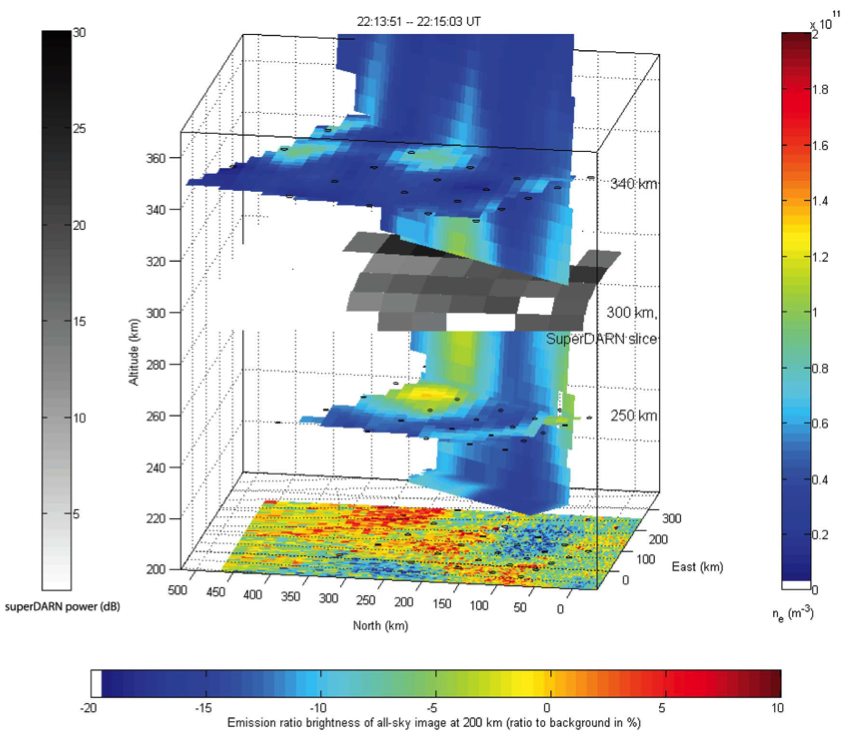
\includegraphics[width=4.0in]{patches}
%% where an .eps filename suffix will be assumed under latex, 
%% and a .pdf suffix will be assumed for pdflatex; or what has been declared
%% via \DeclareGraphicsExtensions.
%\caption{Example of polar cap patches seen in RISR and SuperDARN, from \citep{Dahlgren:2012dq}}
%\label{fig:patches}
%\end{figure}
%
%Large horizontal gradients also occur during geomagnetic storms which can produce large flows.  This can create large disparities in Ion temperature as heating is occurring \citep{Zettergren:2008ba,semeter:plasmatransport2012}.  During these storms ion temperatures can go from 500$^\circ$ K to over 1500$^\circ$ K in the order of kilometers.
%
%These high gradient events can cause some unpredictable errors where two plasma population interface.  These errors can be quite complex due to the nonlinear nature of the inversion process\citep{Vallinkoski1990665}.  Similar behavior has been observed during times of auroral turbulence where shear flows seems to have caused non isotropic temperature measurements\citep{knudsen1993}. 
%%\subsection*{Small Structure Events}
%%\citep{semeter2010CI}
%
%\subsubsection{Dynamic Phenomena}

The resulting ionospheric structures vary over several decades of spatio-temporial scales, creating difficult sampling problems for sensors tasked with measuring them. There are a number of different mechanisms behind this structuring. Auroral precipitation produces variations on a sub kilometer scale variation in electron density perpendicular to magnetic field \citep{Semeter:2005fo}. Convective transport induced by electric fields ($\vec{E}\times\vec{B}$ drift \citep{chen1984introduction}) can cause differential flow velocities and striates the plasma \citep{Tsunoda:1988ul}. This transport can also induce gradient-drift instabilities which have the ability to produce a wide range of irregular structures \citep{GRL:GRL52468}. Field aligned currents (Birkeland currents) can lead to density depletions caused by downward current channels (upflowing ions) \citep{Perry:2015jf}.

Two examples from the literature are examined to highlight the challenges associated with trying to reconstruct the plasma parameters.
The events shown in \citep{Semeter:2005fo} are referred to as a poleward boundary intensification (PBI). This occurs when the auroral oval breaks into two separate rings which show a demarcation of different field line configurations in the magnetosphere. The auroral ring closer to the magnetic pole shows a number of strong pulsations seen in both optical and radar data. The radar reconstruction of this event shown in Figure~\ref{fig:Sampling} shows large enhancements in electron density perpendicular to the ground. The enhancements are rapidly moving, which significantly impacts reconstruction ambiguity by how one processes the data. In this case the researchers found if they integrated fewer pulses per position and allowed for a greater variance in the data they could observe finer column structuring within the enhancement. The simple change in the processing yields significantly different interpretations of the true space-time variability of these structures. More problematic is that the researchers, at the time, did not have a frame work to evaluate the fidelity of their results.
% * <mhirsch@bu.edu> 2016-11-14T18:07:03.028Z:
%
% ground_\perp or B_\perp?
%
% ^.

\begin{figure}[htb]
  \begin{minipage}[t]{0.49\linewidth}\centering
    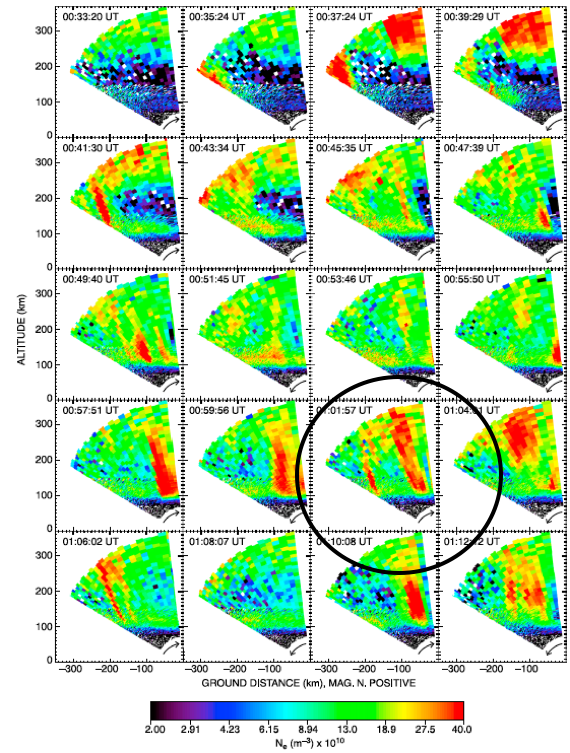
\includegraphics[width=7cm]{pbiall}
    \medskip
    \centerline{(a)}
  \end{minipage}\hfill
  \begin{minipage}[t]{0.49\linewidth}\centering
    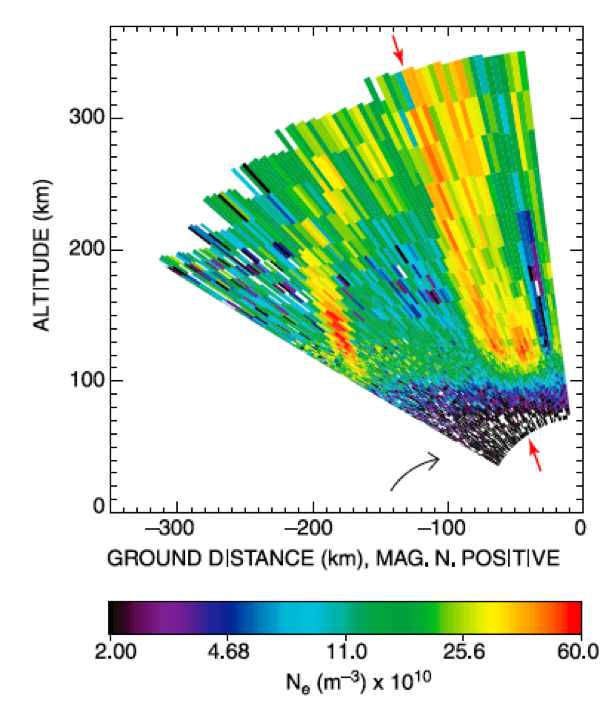
\includegraphics[width=7cm]{pbifast}
    \medskip
    \centerline{(b)}
  \end{minipage}
  \caption{Different views of a PBI event as seen in \citet{Semeter:2005fo}: (a) Data from the Sondrestrøm ISR processed at 5 seconds; and (b) the same data from the circled frame in a but processed at 2 seconds.}
  \label{fig:Sampling}
\end{figure}

The second example event is a sun-aligned auroral arc~\citep{Perry:2015jf}. These arcs are created by Field Aligned Currents (FAC) from the magnetosphere. The evidence of these structures are electron and ion temperature enhancements coincident with electron density depletions next to density enhancements. These structures also are in motion, which can create ambiguities (blurring) in the measurement process as the plasma moves through the field of view. A plasma parameter distribution associated with this type of auroral arc can be seen in Figure~\ref{fig:mzsim}.
\begin{figure}[!t]
\centering
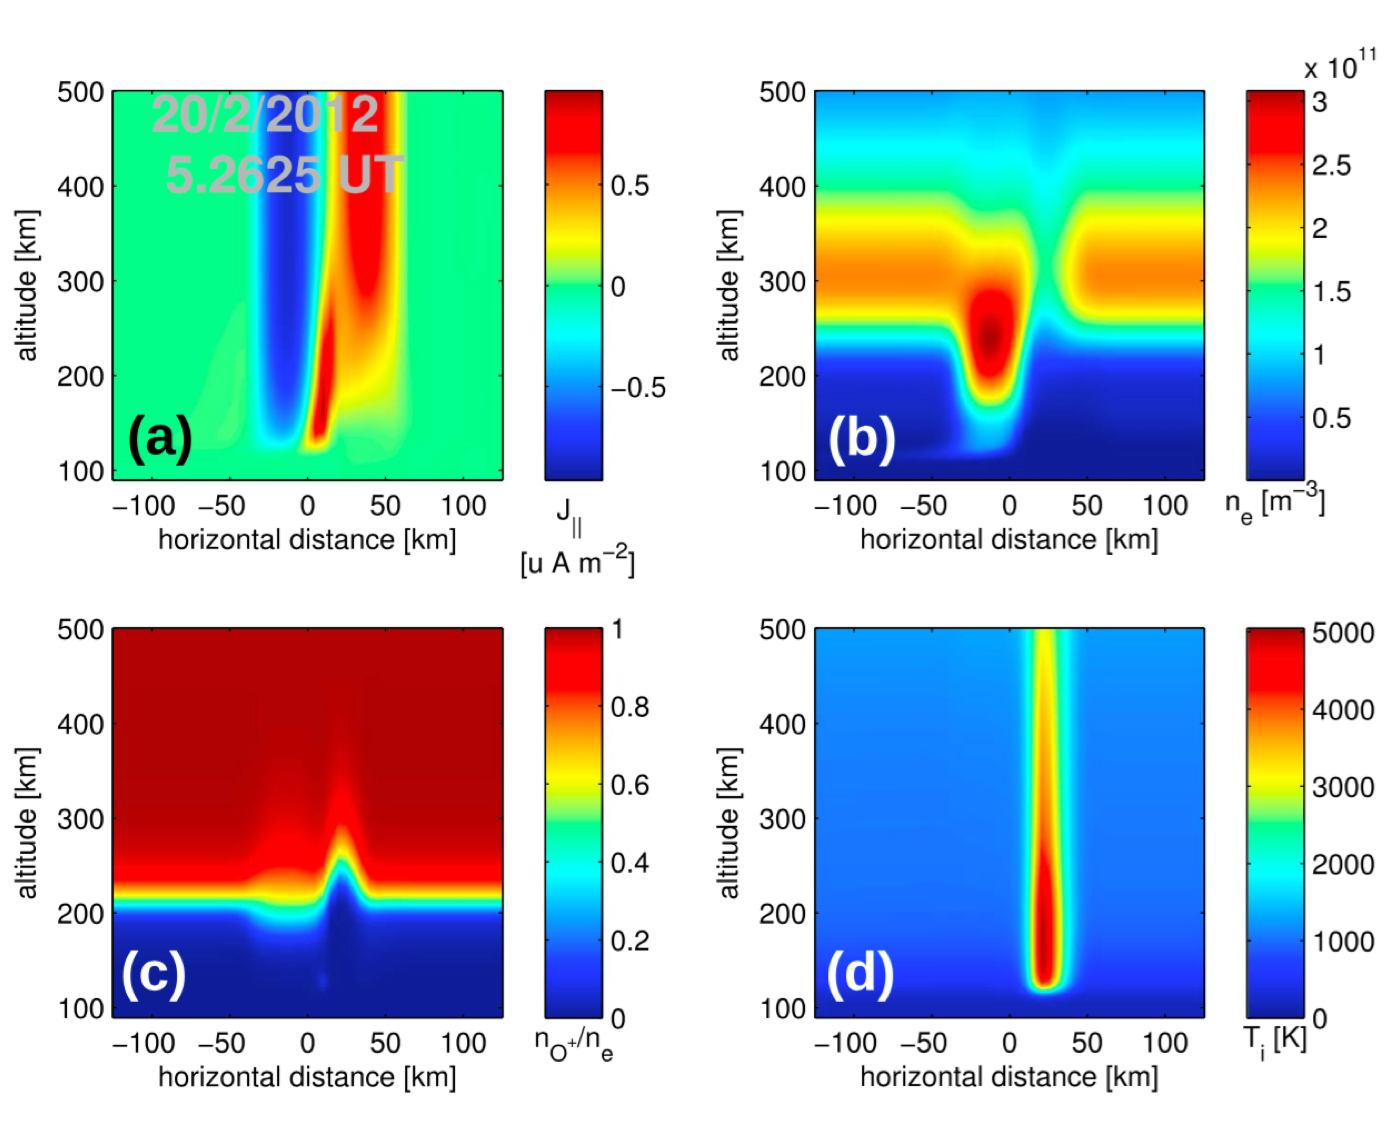
\includegraphics[width=5.0in]{MZsim}
\caption{Plasma parameters used in~\citet{Perry:2015jf} from a multi-fluid model~\citep{semeter:plasmatransport2012} simulating the impact of a field align current. }
\label{fig:mzsim}
\end{figure}


In order to measure these highly structured events using ESA ISR systems researchers would created highly dense beam modes and recreate 3-D interpolations of the data \citep{Dahlgren:2012dq,dahlgren2012di}. Often the radar data sets would be plotted with measurements from corresponding sensors such as in Figure~\ref{fig:risrfusion}. This sort of sensor fusion technique can give an overall picture to the process that is taking place. If ambiguities in each sensor are not understood properly though incorrect interpretations of the physics could take place or lowering the chance of properly testing theoretical models. 

\begin{figure}[!t]
\centering
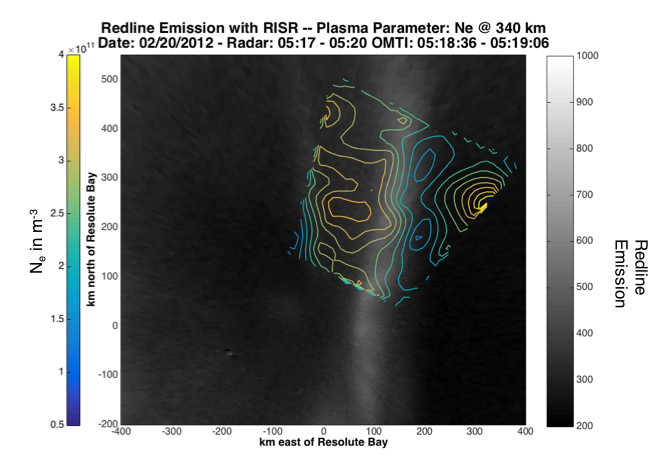
\includegraphics[width=4.0in]{risrfusion}
\caption{Combination of red-line emission data, in gray scale, and an interpolated electron density slice at 340 km from RISR. The red-line emission corresponds with high gradient within the electron density.}
\label{fig:risrfusion}
\end{figure}
%There are also a large number of dynamics and structure found in many auroral events. Using the AMISR system to create volumetric reconstruction of the electron density \citep{Semeter2009738} helped show variability of these events. Figure \ref{fig:eregionact} shows an example of one of these reconstructed events.  Again the like before the researchers again showed the variability during these events by changing the number of pulses integrated and found a large difference in the visible structure.
%\begin{figure}[!t]
%\centering
%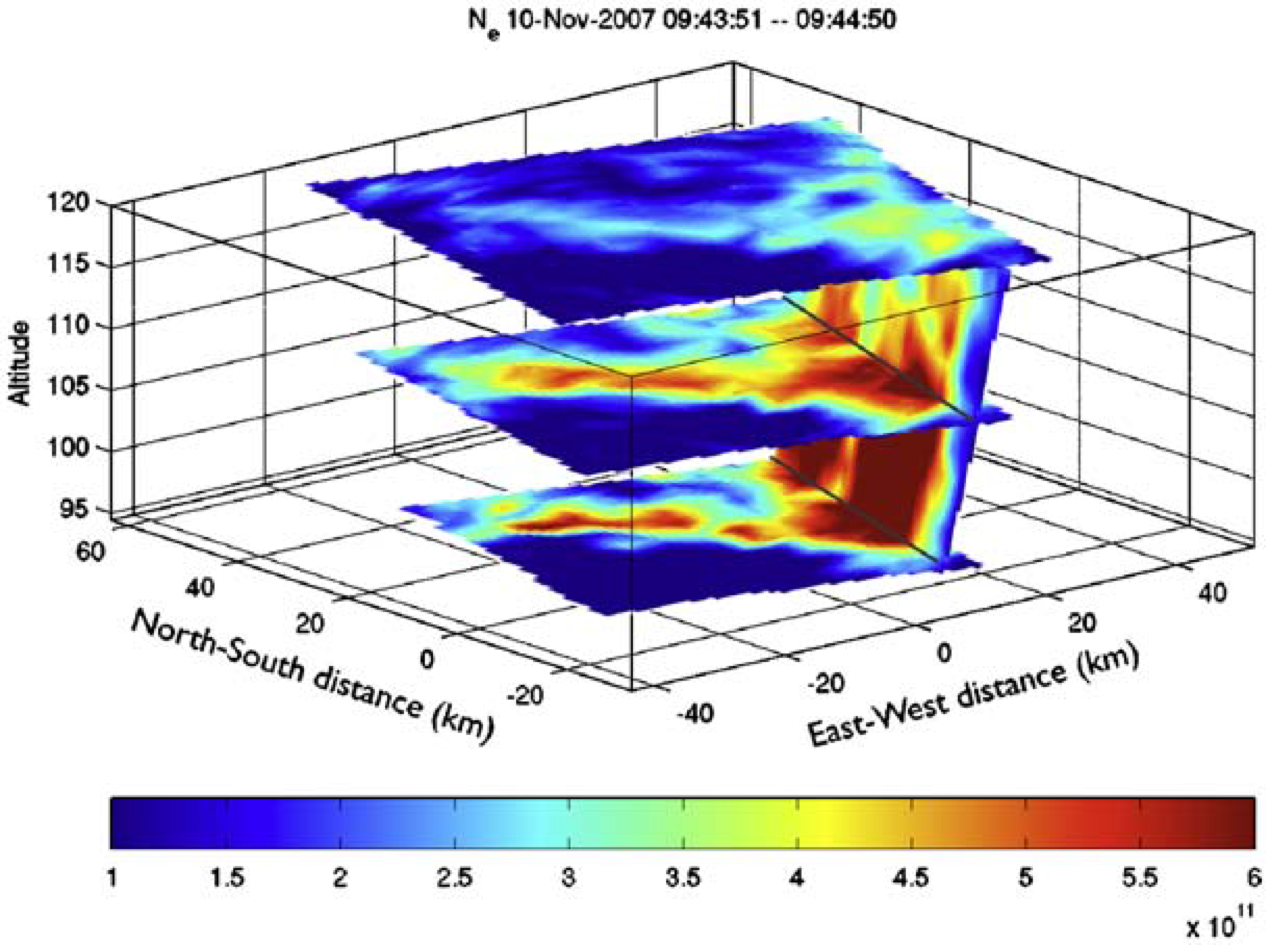
\includegraphics[width=4.0in]{threedamisr}
%\caption{A volumetric reconstruction from AMISR system, from \citep{Semeter2009738}. The reconstruction is of the E-region ionosphere during a auroral precipitation event i.e. electrons following the magnetic field lines of the earth to the lower ionosphere and creating ionization.}
%\label{fig:eregionact}
%\end{figure}
%\subsubsection{High Speed Events}
%At times the ionosphere can be come locally unstable this can create a number of different types of turbulent events. Langmuir turbulence can create coherent structures that will be detected by ISR systems \citep{akbari:2013lt}.  These structures change on the order of one pulse repetition interval of the radar.
%
%Resolving these high speed events are of great interest but also a challenge.  In ISR systems each pulse is used as a sample of a spectral averaging procedure.  It is assumed that these spectrums are identical independent samples.  If spectrum changes during this time, errors in the measurement could take place.  These errors are often unpredictable due to the nonlinear fitting used to fit the spectrum with the plasma parameters.
 %\citep{Dahlgren:2013ip}
%In the past researchers have studied errors associated with different plasma distributions mixing together.  These errors can be quite complex due to the nonlinear nature of the inversion process\citep{Vallinkoski1990665}.  Similar behavior has been observed during times of auroral turbulence where shear flows seems to have caused non isotropic temperature measurements\citep{knudsen1993}. 

\subsubsection{Objectives related to the Phenomena of the Ionosphere}
An important ISR use case is obtaining accurate reconstructions of ionospheric plasma parameters and research creates a framework researchers can use to improve their experiment planning. This framework includes an ISR data simulator useful for trying different experiment setups and reconstruction methods. The simulator can be used as a way to understand possible ambiguities that may arise from experiments if plasma parameters from a physical model are available, such as in~\citet{Perry:2015jf}. The ISR simulation outputs possible measurements given a set of input plasma parameters, including though from fully consistent physical models. In this thesis examples of the simulator are show using phantoms derived from plasma parameters those shown in Figures~\ref{fig:Sampling} and~\ref{fig:mzsim}. 


\subsection{Image Reconstruction}
\label{sec:imgrec}
Inverse theoretic image reconstruction gives engineers and scientists a robust framework to determine the state of system parameters given a set of observations \citep{menke2012geophysical,Vogel:2002:CMI:581830,Karl:2005jy}. This sort of framework has been applied to numerous problems in science and engineering from X-Ray computed tomographic scanning \citep{kak1988principles} to synthetic aperture radar \citep{1456966}. In this thesis we will use this framework and techniques to improve the quality of the plasma parameter estimates from ISR.

Image reconstruction and inverse theory create a framework to reconstruct a set of parameters given a set of data using knowledge of the forward model. Using the notation found in \citet{menke2012geophysical}, a general inverse problem is to find $\mathbf{m}$ such that,
\begin{equation}
\label{eqn:invprob}
\mathbf{d}=\mathbf{g}(\mathbf{m})
\end{equation}
where $\mathbf{d}$ is the observable data and $\mathbf{g}$ is the operator that changes the unobservable parameters $\mathbf{m}$ to the data space. 

Equation \ref{eqn:invprob} gives the most general form of these problems; unfortunately this can be very difficult to solve without further assumptions. Techniques often used to solve inverse problems specify a constraint on the operator $\mathbf{g}$, such that it has to be well-posed \citep{0266-5611-4-4-010}. Still, there are ways to expand the utility of these techniques by adding constraints to the inversion method or regularizing the solution \citep{Vogel:2002:CMI:581830,Karl:2005jy}.

ISR systems have been analyzed in this format, albeit mainly for a single beam \citep{Vierinen:2012ve}. ISR can be posed as a general inverse problem because of the non-linear operation that translates the plasma parameters to the space of possible ACFs. Two schools of thought have emerged in the community on how to constrain these inversions. The first, full profile analysis, uses plasma parameter constraints, which can give physical constraints to the inversion thereby improving the outcome \citep{hysell2008,RDS:RDS3308}. The second set of techniques apply constraints on the estimated ACFs \citep{Virtanen:20082vx,nikoukar2008}, which is less expensive computationally but can create ACFs that cannot be reconciled with physics-based incoherent scatter (IS) theory.

\subsubsection{Objectives related to the image reconstruction}
This thesis will express 3-D ISR in the language of inverse theory and develop a mathematical framework for this specific measurement process. The utility of this framework will be shown in two main ways; first, how ISR data can be improperly interpreted, and secondly, develop techniques to improve the accuracy of the reconstruction of plasma parameters.

\subsection{Outline of dissertation}

Chapter \ref{chapter:isrproc} will go into the background of ISR signal processing. This will begin by developing the basic signal model, showing processing steps from complex voltage samples to plasma parameter measurements.

Chapter 3 will show the derivation of the space-time ambiguity function. This will allow posing of a reconstruction problem for the field of three dimensional plasma parameters in the language of inverse theory. The impact of motion of ionospheric plasma on the ambiguity be shown through plots of the ambiguity but also using real ISR data.  

Chapter 4 contains a discussion of the framework behind the Simulator for ISR (SimISR). This simulator can create complex voltage samples and process the data. This can help plan experiments in the future. Experiments used to validate model predictions require a rigorous understanding of the measurement process. This will also include examples of simulated data to show the capabilities of this framework.

Chapter 5 will detail an inversion method that has been developed to reduce the impact of the space-time ambiguity. This inversion method allows for plasma parameter reconstructions along the frame of reference of the moving plasma assuming a stationary morphology. This takes advantage of the multi-beam measurement capability of ESA ISRs to create high-fidelity image of the moving plasma parameters. This will remove motion blur and could allow researchers to get a better measurements of spatiotemporal structure of the ionosphere. 

\section{Novel Contributions}
Specific novel contributions of this research are summarized below.

\begin{enumerate}
\item Development of a theoretical framework for the forward model of 3-D ISR plasma parameter reconstructions.
\item Creating a framework for full simulation of an ISR system yielding synthetic complex voltages.
\item Construction of a software package, named SimISR, where code derived from previously mentioned simulation framework has been made available to other researchers.
\item Detailed analysis of the simulation framework using SimISR along with example applications for this new tool.
\item A new method for inverting the space-time ambiguity in the frame of reference of the moving plasma.
\item Use of SimISR to create realistic data and application of the new inversion method to assess its potential for use in ISR experiments.
\end{enumerate}